\frame{\frametitle{Vorbedingungen MediaWiki}
\begin{block}{Webserver}
\begin{itemize}
        \item Wir gehen von einem Apache-Webserver aus, der aus den Repositories gezogen wird.  \pause
        \item \texttt{sudo apt-get install apache2} \pause
\end{itemize}
\end{block}

\begin{block}{PHP}
\begin{itemize}
        \item Wir nutzen die Quellen zur Installation.  \pause
        \item \texttt{sudo apt-get install php5} \pause
\end{itemize}
\end{block}

\begin{block}{MySQL}
\begin{itemize}
        \item Wir nutzen die Quellen zur Installation vom MySQL-Server.  \pause
        \item \texttt{sudo apt-get install mysql-server}
\end{itemize}
\end{block}

}

\frame{\frametitle{Installation MediaWiki Teil I}

\begin{block}{MediaWiki}
\begin{itemize}
        \item Es ist ratsam, jeweils die aktuelleste Version direkt vom Hersteller zu beziehen.  \pause
        \item \url{http://www.mediawiki.org/wiki/Download/de} (zurzeit aktuellste Version 1.160 - 12.1 MB schwer) \pause
        \item Der Einfachheit halber nutzen wir ein Unterverzeichnis im Standard-Verzeichnis des Apaches und verzichten auf das Einrichten einer Subdomain. \pause
        \item \texttt{/var/www/wiki} \pause
        \item Dann \url{http://servername.tld/wiki} mit dem Browser ansteuern
\end{itemize}
\end{block}

}

\frame{\frametitle{Installation MediaWiki Teil II}

\begin{block}{Site einrichten}
        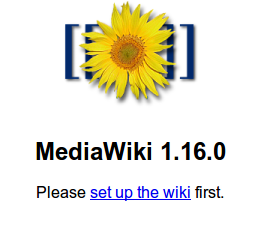
\includegraphics[scale=0.5]{wiki-logo.png}
\begin{itemize}
        \item Auf "Please set up the wiki first" klicken.\pause
        \item Es folgt eine Fehlermeldung "Can't write config file, aborting" mit Anweisungen, das Problem zu lösen.\pause
        \item Fehler in Ordnung bringen und den Wizard erneut starten.

\end{itemize}
\end{block}

}

\frame{\frametitle{Installation MediaWiki Teil III}

\begin{block}{Site einrichten}
\begin{itemize}
        \item Allfällige Fehler beim Ausführen des Wizards beachten.\pause
        \item Formular ausfüllen und \textbf{richtige} Sprache wählen ;-)
        \end{itemize}
		
\includegraphics[scale=0.5]{ch-de.png}
\begin{itemize}
        \item MySQL-Datenbank gemäss Formulardaten erstellen.\pause
        \item Wer möchte, kann das via Browser mit \texttt{phpmyadmin} erledigen.\pause
        \item Das Paket lässt sich mit \texttt{sudo apt-get install phpmyadmin} leicht installieren.
        \item Das Tool ist dann via Standard-Site per Browser erreichbar: \url{http://servername.tld/phpmyadmin}
\end{itemize}
\end{block}

}

\frame{\frametitle{Installation MediaWiki Teil IV}

\begin{block}{Site einrichten}
\begin{itemize}
        \item Das Wiki aufrufen\pause
        \item Fehler \texttt{To complete the installation, move config/LocalSettings.php to the parent directory.} beheben. \pause
        \item Die Konfigurationsdatei \texttt{LocalSettings.php} muss in den Wurzelordner der Website verschoben werden.\pause
        \item Damit läuft das Wiki. Bravo!\pause
        \item Wir schauen uns nun ein paar kosmetische Aenderungen am Wiki an.
\end{itemize}
\end{block}

}

\frame{\frametitle{Das "fertige" MediaWiki}

		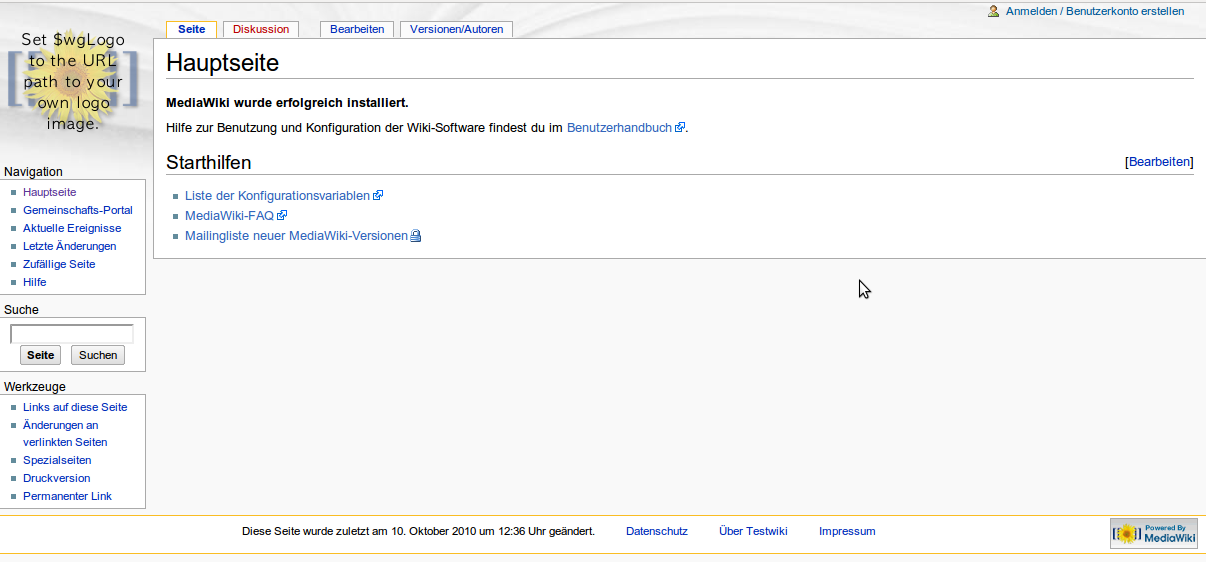
\includegraphics[scale=0.25]{wiki-view.png}

}

\frame{\frametitle{Kosmetischen Anpassungen}

\begin{block}{Logo und andere Einstellungen}
\begin{itemize}
        \item Die wichtigsten Einstellungen sind in der zuvor verschobenen Datei \texttt{LocalSettings.php} untergebracht. \pause
        \item So auch das Logo, beziehungsweise dessen Pfad. \pause
        \item \texttt{\$wgLogo} ist für den Pfad zum Bild zuständig. \pause
        \item Der Standard-Titel ist unschön, da logische Titel dafür verwendet wird. Mit der Erweiterung \texttt{NOTITLE} kann der Titel entfernt werden.
        \item Link zur Erweiterung \url{http://www.mediawiki.org/wiki/Extension:NoTitle}
\end{itemize}
\end{block}

}

\frame{\frametitle{Benutzer Anpassungen (Zugriffe)}

\begin{block}{Benutzer}
\begin{itemize}
        \item Das MediaWiki ist eine kollaborative Software. Jeder soll lesen und schreiben können. \pause
        \item Das ist aber nicht immer erwünscht. Im Verzeichnis \texttt{includes} gibt es die Datei \texttt{DefaultSettings.php}. \pause
        \item Das Array \texttt{\$wgGroupPermissions} muss entsprechend bearbeitet werden. \pause
\end{itemize}
\end{block}

}